\lhead{
\includegraphics[height=1cm]{Logos And Group/LHCb_Logo.png}}
\chead{Hinweise zur Benutzung des Quark-Puzzles}
\rhead{
\includegraphics[height=1cm]{Logos And Group/University of Bonn_logo.png}}
\begin{document}
\hfill\textit{Zur Verwendung für Vermittler*innen und Lehrpersonen}
\section*{Hinweise zum 3d-Druck des Quark-Puzzles}
Sie haben die \texttt{.stl}-Dateien heruntergeladen und möchten nun das Quark-Puzzle drucken. Beachten Sie folgende Hinweise:
\begin{enumerate}\setcounter{enumi}{-1}
    \item Entscheiden Sie welche Flavours Sie benötigen. Aus physikalischer Perspektive ergibt es Sinn eine höhere Anzahl von up- und down- Quarks zu drucken, als bottom- oder top-Quarks.\setcounter{enumi}{-1}
    \item Beachten Sie, dass Sie alle sechs Farben min. einmal drucken. Ansonsten können Sie keine (farbneutralen) Hadronen bauen. \setcounter{enumi}{-1}
    \item Beachten Sie, dass die Druckfarbe der Farbe der Farbladung entsprechen sollte. Stellen Sie sicher, dass Sie über die entsprechenden Farben/Filamente verfügen. \\ \,~Hinweis: Die Druckfarbe ist im Dateinamen und auf der Form vermerkt, \\ \,~Hinweis: Es gilt: Antiblau $=$ Gelb, Antirot $=$ Cyan/Hellblau, Antigrün $=$ Magenta/Pink. \\ \,
    \hline 
    \item Importieren Sie in dem Herstellerprogramm des 3d-Druckers eine der \texttt{.stl}-Dateien.  Verkleinern Sie die Form \textbf{relativ} auf eine Größe von \textbf{ca. 32-40\,mm}. Legen Sie das Quark   \textbf{mit der Seite des Flavours} auf den Grund der Druckebene:
\end{enumerate}
\begin{center}
  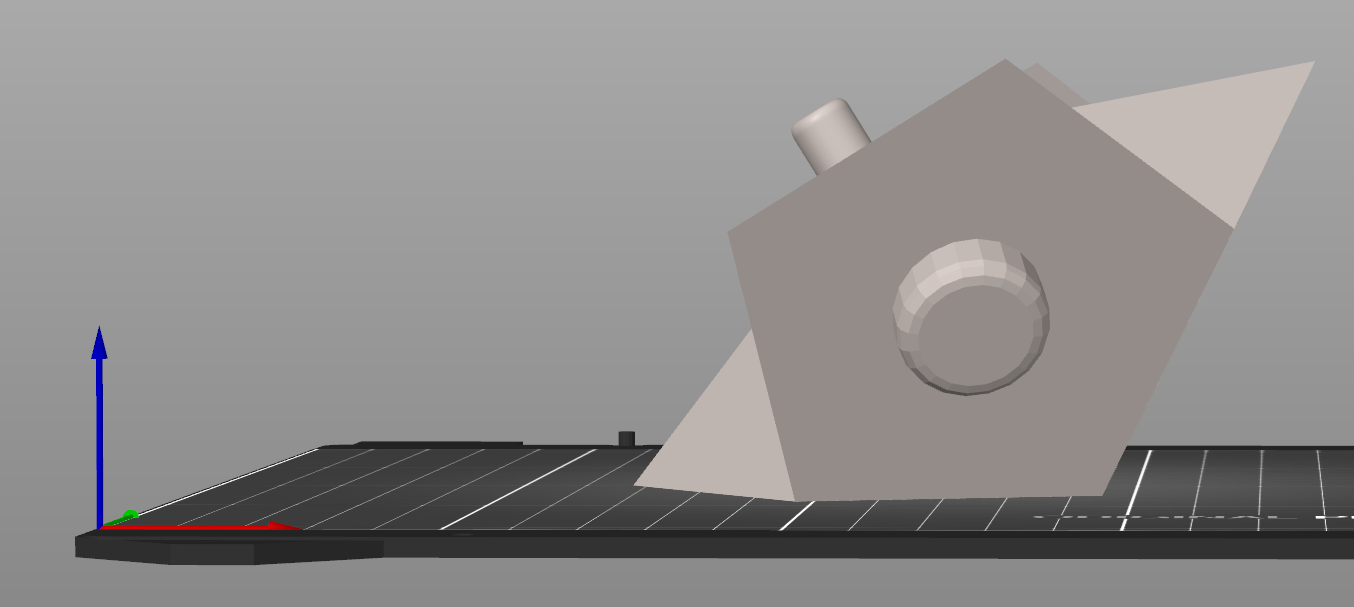
\includegraphics[width=0.5\textwidth]{Pictures Quark Puzzle/2023-11-01 15_13_48-Start.png}  
\end{center}
\begin{enumerate}\setcounter{enumi}{1}
    \item Wiederholen Sie das Procedere für alle gewünschten Quarks der entsprechenden Druckfarbe. Verwenden Sie dabei den \textbf{gleichen Verkleinungsfaktor} wie zuvor.  Aktivieren Sie Stützen und drucken Sie die Quarks der entsprecheden Farbe aus. Das Ergebnis könnte für die Farbladung \emph{grün} wie folgt aussehen:
    

\end{enumerate}
\begin{center}
  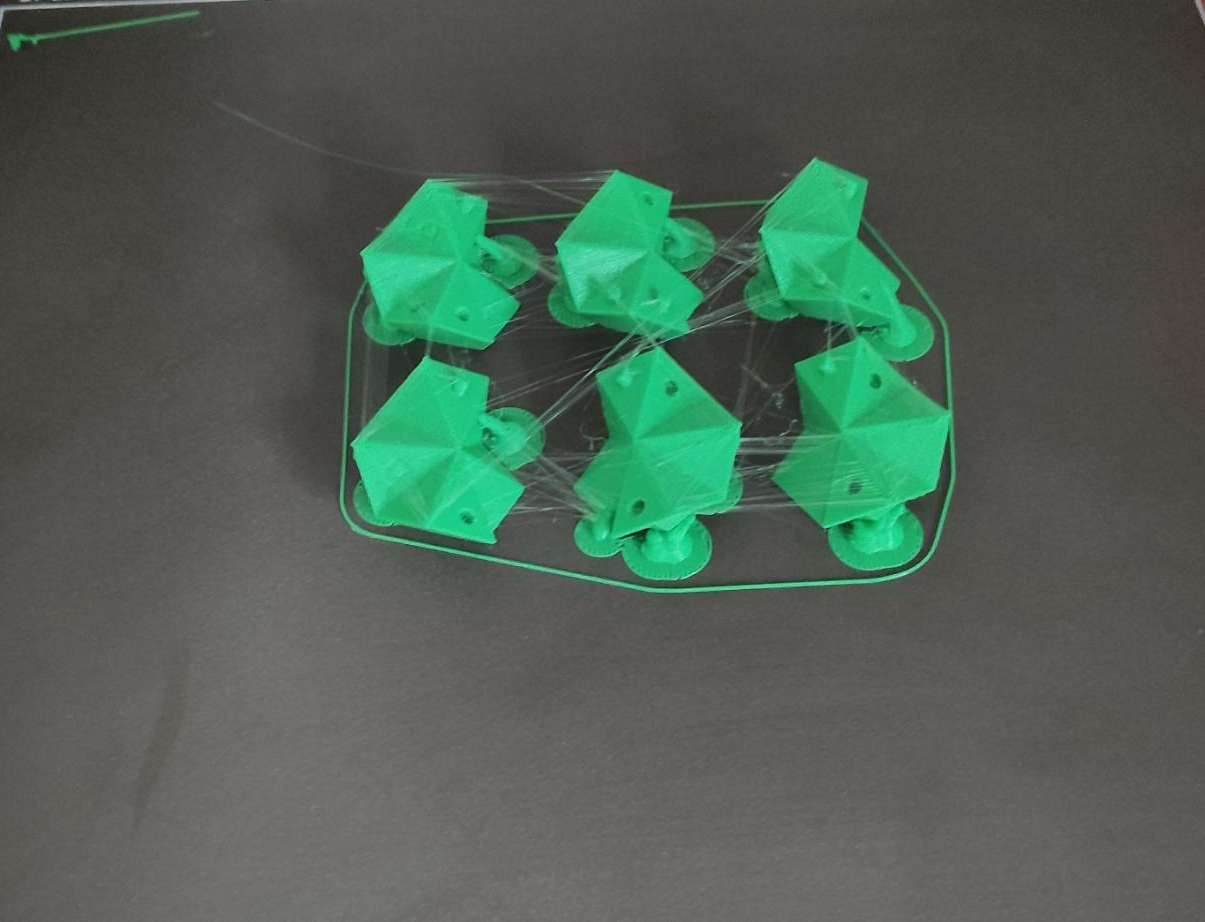
\includegraphics[width=0.5\textwidth]{Pictures Quark Puzzle/IMG_2108.JPG}  
\end{center}
\begin{enumerate}\setcounter{enumi}{2}
     \item Wiederholen Sie den Schritt 1 und 2 für alle Farben, \textbf{benutzen Sie den gleichen Verkleinerungsfaktor} und tauschen Sie ggf. das Filament Ihres Druckers.
     \item Sie sind fertig, entfernen Sie zuletzt Stützen mit einem Schraubenzieher oder mit einer Nagelpfeile. 
   
\end{enumerate}
\, \\ 
Anmerkungen:
\begin{itemize}
    \item Für Drucke größer als 40\,mm halten die Quarks nicht mehr perfekt zusammen. Eine Version hierfür ist geplant.
    \item Die einzelnen Farbvarianten besitzen leicht unterschiedliche Größen, vermeiden Sie daher die Verkleinerung auf absolute Werte und benutzen Sie den immer gleichen Verkleinerungsfaktor!
\end{itemize}

\subsection*{Kontakt* - LHCb Bonn}

\begin{table}[h]
    \centering
    \begin{tabular}{ccc}
        Lukas Julian Exner & Klaas Padeken & Sebastian Neubert  \\
      \textsf{\ding{41} \footnotesize \ding{}  exner@hiskp.uni-bonn.de} & \textsf{\ding{41} \footnotesize  padeken@hiskp.uni-bonn.de} & \textsf{\ding{41} \footnotesize  neubert@hiskp.uni-bonn.de}
    \end{tabular}
    \label{tab:my_label}
\end{table}
\textbf{*} Bitte nur Lukas Julian Exner bei Fragen bzgl. des Drucks anschreiben.

\end{document}
